\documentclass{minimal}
%\documentclass[conference]{IEEEtran}
\usepackage{pgf}
\usepackage{tikz}
\usepackage[utf8]{inputenc}
\usetikzlibrary{arrows,automata}
\usetikzlibrary{positioning}


\tikzset{
	state/.style={
		rectangle,
		rounded corners,
		draw=black, very thick,
		minimum height=2em,
		inner sep=2pt,
		text centered,
	},
}

\begin{document}
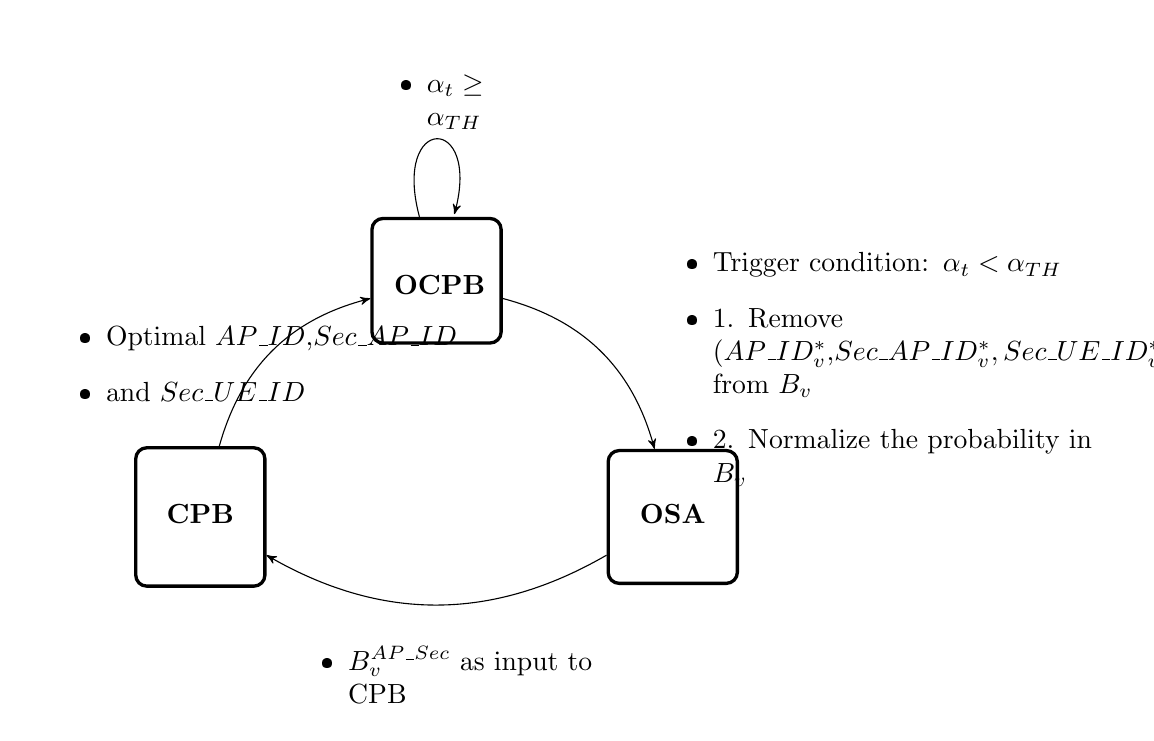
\begin{tikzpicture}[->,>=stealth']

 % First node
 % Use previously defined 'state' as layout (see above)
 % use tabular for content to get columns/rows
 % parbox to limit width of the listing
 \node[state,text width=1.5cm] (CPB) 
 {\begin{tabular}{l}
 	\\[0.5em]
  \textbf{CPB}\\
  \parbox{2cm}{
  }\\[0.5em]
  %\textbf{QueryAdjust}\\
  %\parbox{4cm}{Wähle neue Spreizsequenz}
 \end{tabular}};

 % Next node: OCPB
 \node[state,       % layout (defined above)
 node distance=3cm,     % distance to QUERY
 text width=1.5cm,        % max text width
 right of=CPB,        % Position is to the right of QUERY
 yshift=+3cm] (OCPB)    % move 3cm in y
 {%                     % posistion relative to the center of the 'box'
 \begin{tabular}{l}     % content
   \\[0.5em]
  \textbf{OCPB}\\
  \parbox{2.8cm}{}
  %\parbox{2.8cm}{Paralleles Entspreizen aller Sequenzen aus $T_P$}
 \end{tabular}  	\\[0.5em]
 };

 % STATE ACK
 \node[state,
 right of=OCPB,
 node distance=3cm,
 yshift=-3cm,
 text width=1.5cm] (OSA) 
 {	
 \begin{tabular}{l}
 \\[0.4em]
  \textbf{OSA}\\
  \parbox{2.8cm}{ }
  \\[0.4em]
 \end{tabular}

 };

 
 % draw the paths and and print some Text below/above the graph
 \path (CPB) edge[bend left=30]  node[anchor=south,above,text width=6cm,yshift=-2.2em]
                   {
                   \begin{itemize}
                    \item Optimal $AP\_ID$,$Sec\_AP\_ID$
                    \item and $Sec\_UE\_ID$ 
                   \end{itemize}
                   } (OCPB)
 (OCPB) edge [bend left=30] node  [anchor=east,right,text width=6cm,,xshift=1.2em]
 {
 	\begin{itemize}
 	\item Trigger condition: $\alpha_{t}<\alpha_{TH}$
 	\item 1. Remove $(AP\_ID^{*}_{v}$,$Sec\_AP\_ID^{*}_{v},Sec\_UE\_ID^{*}_{v})$ from $B_{v}$
 	\item 2. Normalize the probability in $B_{v}$
 	\end{itemize}
 }  (OSA)
 (OCPB)  edge[loop above]    node[anchor=south,above,text width=2cm]
 {
 	\begin{itemize}
 	\item $\alpha_{t}\geq \alpha_{TH}$
 	\end{itemize}
 }         (OCPB)
 
 (OSA)  edge[bend left=30] node[anchor=north,below,text width=4cm]
                  {\begin{itemize}
                   \item $B_{v}^{AP\_Sec}$ as input to CPB
                  \end{itemize}
                  } (CPB)
 ;
\end{tikzpicture}
\end{document}